\documentclass{report}

\usepackage{amsmath, amssymb}
\usepackage{ctex}
\usepackage[total={7in, 9.6in}]{geometry}
\usepackage{enumitem}
\usepackage{multicol}
\usepackage{tikz}

\newcommand{\sol}{\vspace{0.2cm}\textbf{解}:}
\pagenumbering{gobble}

\begin{document}
\setcounter{chapter}{8}
\setcounter{section}{2}

\section{倍角及半角的三角函数}

\allowdisplaybreaks
    \begin{enumerate}[leftmargin=*]
        \item 试证公式 $\sin \theta=\dfrac{2 t}{1+t^2}, \cos \theta=\dfrac{1-t^2}{1+t^2}$, 其中 $t=\tan \dfrac{\theta}{2}$。然后据此, 或用其他方法,证明: 若 $0 \leq \theta \leq \dfrac{\pi}{2}$, 则 $\dfrac{1-\sin \theta}{1+\sin \theta}=\tan ^2\left(\dfrac{\pi}{4}-\dfrac{\theta}{2}\right)$ 及 $1 \leq \dfrac{1+\sin \theta+\cos \theta}{1+\cos \theta} \leq 2$。
        
        \sol{}
        
        Let $t=\tan \dfrac{\theta}{2}$, then $\tan \theta=\dfrac{2 t}{1-t^2}$,
       \begin{center}
        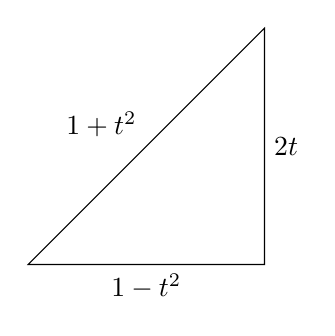
\begin{tikzpicture}
            \draw (0,0) -- (3,0) -- (3,3) -- cycle;
            \node at (3, 1.5) [right] {$2t$};
            \node at (1.5, 0) [below] {$1 - t^2$};
            \node at (1.5, 1.5) [above left] {$1 + t^2$};
        \end{tikzpicture}
       \end{center}
        \begin{align*}
            \sin \theta &= \dfrac{2t}{1+t^2},\\
            \cos \theta &= \dfrac{1-t^2}{1+t^2} & \blacksquare
        \end{align*}
        \begin{align*}
            L.H.S. &= \dfrac{1-\sin \theta}{1+\sin \theta} = \dfrac{1-\dfrac{2t}{1+t^2}}{1+\dfrac{2t}{1+t^2}} = \dfrac{1+t^2-2t}{1+t^2+2t} = \dfrac{(1-t)^2}{(1+t)^2}\\
            R.H.S. &= \tan^2\left(\dfrac{\pi}{4}-\dfrac{\theta}{2}\right) = \left(\dfrac{\tan\dfrac{\pi}{4}-\tan\dfrac{\theta}{2}}{1+\tan\dfrac{\pi}{4}\tan\dfrac{\theta}{2}}\right)^2 = \left(\dfrac{1-\tan\dfrac{\theta}{2}}{1+\tan\dfrac{\theta}{2}}\right)^2 = \dfrac{(1-t)^2}{(1+t)^2}
        \end{align*}
        $\because L.H.S. = R.H.S.$, hence proved. \hfill $\blacksquare$
        \begin{align*}
            \dfrac{1+\sin \theta+\cos \theta}{1+\cos \theta} &= \dfrac{1+\dfrac{2t}{1+t^2}+\dfrac{1-t^2}{1+t^2}}{1+\dfrac{1-t^2}{1+t^2}}\\
            & = \dfrac{1+t^2+2t+1-t^2}{1+t^2+1-t^2}\\
            & = \dfrac{2+2t}{2}\\
            & = 1+t\\
            & = 1+\tan\dfrac{\theta}{2}\\
            0 \leq \tan\dfrac{\theta}{2} \leq 1 &\Rightarrow 1 \leq 1+\tan\dfrac{\theta}{2} \leq 2 & \blacksquare
        \end{align*}
        
        \newpage
        \item 从 $\tan \theta=a$ 及 $\cos 2 \theta=b$ 二式中消去 $\theta$, 写出 $a$ 与 $b$ 之间的关系式子。
        
        \sol{}
        \begin{align*}
            \tan\theta &= a\\
            \dfrac{\sin\theta}{\cos\theta} &= a\\
            \sin\theta &= a\cos\theta\\
            \sin^2\theta &= a^2\cos^2\theta\\
            1-\cos^2\theta &= a^2\cos^2\theta\\
            1 &= a^2\cos^2\theta + \cos^2\theta\\
            1 &= (a^2+1)\cos^2\theta\\
            \cos^2\theta &= \dfrac{1}{a^2+1}\\
            \\
            \cos 2\theta &= b\\
            \cos^2\theta - \sin^2\theta &= b\\
            \cos^2\theta - a^2\cos^2\theta &= b\\
            (1-a^2)\cos^2\theta &= b\\
            \cos^2\theta &= \dfrac{b}{1-a^2}\\
            \\
            \dfrac{1}{a^2+1} &= \dfrac{b}{1-a^2}\\
            b &= \dfrac{1-a^2}{1+a^2} & \blacksquare
        \end{align*}
                
        \item 已知 $t=\tan \dfrac{\theta}{2}$, 试证 
        \begin{enumerate}
            \item $\sin \theta=\dfrac{2 t}{1+t^2}$;
            \item $\cos \theta=\dfrac{1-t^2}{1+t^2}$。
        \end{enumerate}

        \sol{}

        Same as question 1. \hfill $\blacksquare$
                
        \item 试证明 $\cos ^2 x+\cos ^2\left(x+\dfrac{2 \pi}{3}\right)+\cos ^2\left(x+\dfrac{4 \pi}{3}\right)=\dfrac{3}{2}$。
        
        \sol{}
        \begin{align*}
            &\ \ \ \cos ^2 x+\cos ^2\left(x+\dfrac{2 \pi}{3}\right)+\cos ^2\left(x+\dfrac{4 \pi}{3}\right)\\
            &= \cos ^2 x + \left[\cos x \cos \dfrac{2 \pi}{3} - \sin x \sin \dfrac{2 \pi}{3}\right]^2 + \left[\cos x \cos \dfrac{4 \pi}{3} - \sin x \sin \dfrac{4 \pi}{3}\right]^2\\
            &= \cos ^2 x + \left[-\dfrac{1}{2}\cos x - \dfrac{\sqrt{3}}{2}\sin x\right]^2 + \left[-\dfrac{1}{2}\cos x + \dfrac{\sqrt{3}}{2}\sin x\right]^2\\
            &= \cos ^2 x + \dfrac{1}{4}\cos ^2 x + \dfrac{3}{4}\sin ^2 x + \dfrac{1}{4}\cos ^2 x + \dfrac{3}{4}\sin ^2 x\\
            &= \dfrac{3}{2}\cos ^2 x + \dfrac{3}{2}\sin ^2 x\\
            &= \dfrac{3}{2}(\cos ^2 x + \sin ^2 x)\\
            &= \dfrac{3}{2} & \blacksquare
        \end{align*}
        
        \item 已知 $\cos y=\dfrac{1}{8}$, 不许查表或用计算机, 求 (i) $\cos 2 y$ 及 (ii) $\cos \dfrac{1}{2} y$ 之值。
        
        \sol{}
        \begin{center}
            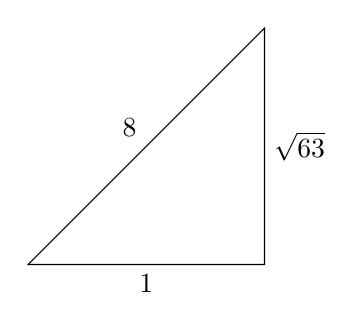
\begin{tikzpicture}
                \draw (0,0) -- (3,0) -- (3,3) -- cycle;
                \node at (3, 1.5) [right] {$\sqrt{63}$};
                \node at (1.5, 0) [below] {$1$};
                \node at (1.5, 1.5) [above left] {$8$};
            \end{tikzpicture}
        \end{center}
        \begin{align*}
            \sin y &= \dfrac{\sqrt{63}}{8} \qquad \cos y = \dfrac{1}{8}\\
        \end{align*}
        \begin{align*}
            \cos 2y &= 2\cos^2 y - 1 = 2\left(\dfrac{1}{8}\right)^2 - 1 = -\dfrac{31}{32}\\
            \cos \dfrac{1}{2}y &= \pm\sqrt{\dfrac{1+\cos y}{2}} = \pm\sqrt{\dfrac{1+\dfrac{1}{8}}{2}} = \pm\sqrt{\dfrac{9}{16}} = \pm\dfrac{3}{4} & \blacksquare
        \end{align*}
                
        \item 试证 $\sin 3 \theta=4 \sin \theta \sin \left(60^{\circ}+\theta\right) \sin \left(60^{\circ}-\theta\right)$。
        
        \sol{}
        \begin{align*}
            L.H.S. = \sin 3\theta &= \sin(2\theta + \theta)\\
            & = \sin 2\theta \cos \theta + \cos 2\theta \sin \theta\\
            & = 2\sin\theta\cos^2\theta + (1-2\sin^2\theta)\sin\theta\\
            & = 2\sin\theta(1-\sin^2\theta) + \sin\theta - 2\sin^3\theta\\
            & = 2\sin\theta - 2\sin^3\theta + \sin\theta - 2\sin^3\theta\\
            & = 3\sin\theta - 4\sin^3\theta\\
            R.H.S. = 4\sin\theta\sin\left(60^{\circ}+\theta\right)\sin\left(60^{\circ}-\theta\right) &= 4\sin\theta\left(\dfrac{\sqrt{3}}{2}\cos\theta + \dfrac{1}{2}\sin\theta\right)\left(\dfrac{\sqrt{3}}{2}\cos\theta - \dfrac{1}{2}\sin\theta\right)\\
            &= 4\sin\theta\left(\dfrac{3}{4}\cos^2\theta - \dfrac{1}{4}\sin^2\theta\right)\\
            & = 3\sin\theta\cos^2\theta - \sin^3\theta\\
            & = 3\sin\theta(1-\sin^2\theta) - \sin^3\theta\\
            & = 3\sin\theta - 3\sin^3\theta - \sin^3\theta\\
            & = 3\sin\theta - 4\sin^3\theta
        \end{align*}
        $\because L.H.S. = R.H.S.$, hence proved. \hfill $\blacksquare$
                
        \item 试证 $4 \sin ^6 \theta+4 \cos ^6 \theta+3 \sin ^2 2 \theta=4$。
        
        \sol{}
        \begin{align*}
            &\ \ \ 4 \sin ^6 \theta+4 \cos ^6 \theta+3 \sin ^2 2 \theta\\
            &= 4(1-\cos^2\theta)^3 + 4\cos^6\theta + 12\sin^2\theta\cos^2\theta\\
            &= 4(1-3\cos^2\theta + 3\cos^4\theta - \cos^6\theta) + 4\cos^6\theta + 12\sin^2\theta(1-\sin^2\theta)\\
            &= 4 - 12\cos^2\theta + 12\cos^4\theta - 4\cos^6\theta + 4\cos^6\theta + 12\sin^2\theta - 12\sin^4\theta\\
            &= 4 & \blacksquare
        \end{align*}
        
        \item 不许应用对数表或计算机, 试求 $\tan 67 \dfrac{1}{2}^{\circ}$ 之值。
        
        \sol{}
        \begin{align*}
            \tan 67 \dfrac{1}{2}^{\circ} &= \tan\left(\dfrac{135^{\circ}}{2}\right) = \sqrt{\dfrac{1-\cos 135^{\circ}}{1+\cos 135^{\circ}}} = \sqrt{\dfrac{1+\dfrac{\sqrt{2}}{2}}{1-\dfrac{\sqrt{2}}{2}}}\\
            &= \sqrt{\dfrac{2+\sqrt{2}}{2-\sqrt{2}}} = \sqrt{\dfrac{6+4\sqrt{2}}{2}} = \sqrt{3+2\sqrt{2}} \\
            &= \sqrt{2 + 1 + 2\sqrt{2\cdot 1}} = \sqrt{(1+\sqrt{2})^2} = 1+\sqrt{2} & \blacksquare
        \end{align*}
        
        \item 试证 $\dfrac{1-\cos x}{1+\cos x}=\tan ^2 \dfrac{x}{2}$。
        
        然后由上述结果推证 $\tan 15^{\circ}=2-\sqrt{3}$。

        \sol{}
        \begin{align*}
            \dfrac{1-\cos x}{1+\cos x} &= \left(\sqrt{\dfrac{1-\cos x}{1+\cos x}}\right)^2 = \left(\tan\dfrac{x}{2}\right)^2 = \tan^2\dfrac{x}{2} & \blacksquare
        \end{align*}
        \begin{align*}
            \tan 15^{\circ} &= \tan\dfrac{30^{\circ}}{2} = \sqrt{\dfrac{1-\cos 30^{\circ}}{1+\cos 30^{\circ}}} = \sqrt{\dfrac{1-\dfrac{\sqrt{3}}{2}}{1+\dfrac{\sqrt{3}}{2}}}\\
            &= \sqrt{\dfrac{2-\sqrt{3}}{2+\sqrt{3}}} = \sqrt{\dfrac{(2-\sqrt{3})^2}{4-3}} = \sqrt{\dfrac{4-4\sqrt{3}+3}{1}} = \sqrt{7-4\sqrt{3}}\\
            &= \sqrt{7 - 2\sqrt{12}} = \sqrt{4 + 3 - 2\sqrt{4\cdot 3}} = \sqrt{(2-\sqrt{3})^2} = 2-\sqrt{3} & \blacksquare
        \end{align*}
        
        
        \item 已知 $\sin ^2 \theta+6 \sin \theta \cos \theta+9 \cos ^2 \theta \equiv a+b \sin 2 \theta+c \cos 2 \theta$, 试求 $a, b, c$ 之值。据此或其他方法, 试求 $\sin ^2+6 \sin \theta \cos \theta+9 \cos ^2 \theta$ 的极大值和极小值。
        
        \sol{}
        \begin{align*}
            \sin ^2 \theta+6 \sin \theta \cos \theta+9 \cos ^2 \theta &=\dfrac{1 - \cos 2\theta}{2} + 3\cdot 2\sin\theta\cos\theta + 9\left(\dfrac{1 + \cos 2\theta}{2}\right)\\
            &=\dfrac{1 - \cos 2\theta + 9 + 9\cos 2\theta}{2} + 3\sin 2\theta\\
            &=5 + 3\sin 2\theta + 4\cos 2\theta\\
            \therefore\ &a = 5, b = 3, c = 4 & \blacksquare
        \end{align*}
        \begin{align*}
            \dfrac{d}{d\theta}(5 + 3\sin 2\theta + 4\cos 2\theta) &= 6\cos 2\theta - 8\sin 2\theta = 0\\
            \tan 2\theta &= \dfrac{3}{4}\\
            2\theta &= k\pi + \arctan\dfrac{3}{4}\\
            \theta &= \dfrac{k\pi}{2} + \dfrac{1}{2}\arctan\dfrac{3}{4}\\
            \dfrac{d^2}{d\theta^2}(5 + 3\sin 2\theta + 4\cos 2\theta) &= -6\sin 2\theta - 8\cos 2\theta\\
        \end{align*}
        When $k = 0$, $\theta = \dfrac{1}{2}\arctan\dfrac{3}{4}$, $\dfrac{d^2}{d\theta^2} = -6\sin\arctan\dfrac{3}{4} - 8\cos\arctan\dfrac{3}{4} = -3.02 < 0$.

        Hence, the max value is $5 + 3\sin 2\theta + 4\cos 2\theta = 5 + 3\sin\arctan\dfrac{3}{4} + 4\cos\arctan\dfrac{3}{4} = 10$. \hfill $\blacksquare$

        When $k = 1$, $\theta = \dfrac{\pi}{2} + \dfrac{1}{2}\arctan\dfrac{3}{4}$, $\dfrac{d^2}{d\theta^2} = -6\sin\left(\pi + \arctan\dfrac{3}{4}\right) - 8\cos\left(\pi + \arctan\dfrac{3}{4}\right) = 3.02 > 0$.

        Hence, the min value is $5 + 3\sin 2\theta + 4\cos 2\theta = 5 + 3\sin\left(\pi + \arctan\dfrac{3}{4}\right) + 4\cos\left(\pi + \arctan\dfrac{3}{4}\right) = 0$. \hfill $\blacksquare$
        
        \item 证 $\operatorname{cosec} \theta-\cot \theta=\tan \dfrac{1}{2} \theta$。据此或其他方法, 证 $\tan 22 \dfrac{1}{2}^{\circ}=\sqrt{2}-1$。
        
        \sol{}
        \begin{align*}
            \operatorname{cosec}\theta - \cot\theta &= \dfrac{1}{\sin\theta} - \dfrac{\cos\theta}{\sin\theta} = \dfrac{1-\cos\theta}{\sin\theta} = \dfrac{2\sin^2\dfrac{\theta}{2}}{2\sin\dfrac{\theta}{2}\cos\dfrac{\theta}{2}} = \tan\dfrac{\theta}{2} & \blacksquare
        \end{align*}
        \begin{align*}
            \tan 22 \dfrac{1}{2}^{\circ} &= \tan\dfrac{45^{\circ}}{2} = \operatorname{cosec}45^{\circ} - \cot45^{\circ} = \sqrt{2} - 1 & \blacksquare
        \end{align*}

        \item 试证 $8\left(\sin ^6 \theta+\cos ^6 \theta\right)=5+3 \cos 4 \theta$。
        
        \sol{}
        \begin{align*}
            L.H.S. &= 8\left(\sin ^6 \theta+\cos ^6 \theta\right) \\
            &= 8\left((1-\cos^2\theta)^3 + \cos^6\theta\right)\\
            &= 8(1 - 3\cos^2\theta + 3\cos^4\theta - \cos^6\theta + \cos^6\theta)\\
            &= 8(1 - 3\cos^2\theta + 3\cos^4\theta)\\
            R.H.S. &= 5 + 3\cos 4\theta \\
            &= 5 + 3(2\cos^2 2\theta - 1)\\
            &= 2 + 6\cos^2 2\theta\\
            &= 2 + 6(2\cos^2\theta - 1)^2\\
            &= 2 + 6(4\cos^4\theta - 4\cos^2\theta + 1)\\
            &= 2 + 24\cos^4\theta - 24\cos^2\theta + 6\\
            &= 8(1 - 3\cos^2\theta + 3\cos^4\theta)
        \end{align*}
        $\because L.H.S. = R.H.S.$, hence proved. \hfill $\blacksquare$

        \item 已知 $\tan ^2 \alpha=2 \tan ^2 \beta+1$, 试证 $\cos 2 \alpha+\sin ^2 \beta=0$。
        
        \sol{}
        \begin{align*}
            \tan^2\alpha &= 2\tan^2\beta + 1\\
            \dfrac{\sin^2\alpha}{\cos^2\alpha} &= 2\left(\dfrac{\sin^2\beta}{\cos^2\beta}\right) + 1\\
            \dfrac{1-\cos^2\alpha}{\cos^2\alpha} &= 2\left(\dfrac{1-\cos^2\beta}{\cos^2\beta}\right) + 1\\
            \dfrac{1}{\cos^2\alpha} - 1 &= 2\left(\dfrac{1}{\cos^2\beta} - 1\right) + 1\\
            \dfrac{1}{\cos^2\alpha} &= \dfrac{2}{\cos^2\beta}\\
            \cos^2\beta &= 2\cos^2\alpha
        \end{align*}
        \begin{align*}
            \cos 2\alpha + \sin^2\beta &= \cos 2\alpha + 1 - \cos^2\beta\\
            &= 2\cos^2\alpha - 1 + 1 - 2\cos^2\alpha\\
            &= 0 & \blacksquare
        \end{align*}

        \item 已知 $x=\cos \theta$, 式中 $\dfrac{3}{2} \pi<\theta<2 \pi$, 且 $2 \cos \theta-\sin \theta=2$, 证明 $\sqrt{1-x^2}=2(1-x)$。
        
        据此据此或其他方法, 求 $x$ 的值并推证 $\tan 2 \theta=\dfrac{24}{7}$。

        \sol{}
        \begin{align*}
            2\cos\theta - \sin\theta &= 2\\
            2\cos\theta - \sqrt{1-\cos^2\theta} &= 2\\
            2x - \sqrt{1-x^2} &= 2\\
            \sqrt{1-x^2} &= 2(1-x) & \blacksquare
        \end{align*}
        \begin{align*}
            \sqrt{1-x^2} &= 2(1-x) \\
            1-x^2 &= 4(1-x)^2\\
            1-x^2 &= 4(1-2x+x^2)\\
            1 - x^2 &= 4 - 8x + 4x^2\\
            5x^2 - 8x + 3 &= 0\\
            (5x - 3)(x - 1) &= 0\\
            x &= 1 \text{ or } x = \dfrac{3}{5}\\
            \because x &= \cos\theta,\ \theta \in \left(\dfrac{3}{2}\pi, 2\pi\right)\\
            \therefore\ x &> 0 \Rightarrow x = \dfrac{3}{5} & \blacksquare
        \end{align*}
        \begin{center}
            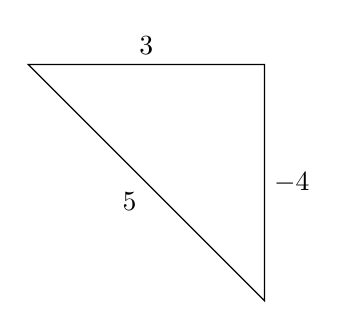
\begin{tikzpicture}
                \draw (0, 3) -- (3, 3) -- (3, 0) -- cycle;
                \node at (1.5, 3) [above] {$3$};
                \node at (3, 1.5) [right] {$-4$};
                \node at (1.5, 1.5) [below left] {$5$};
            \end{tikzpicture}
        \end{center}
        \begin{align*}
            \tan 2\theta &= \dfrac{2\tan\theta}{1-\tan^2\theta} = \dfrac{2\cdot\left(-\dfrac{4}{3}\right)}{1-\left(-\dfrac{4}{3}\right)^2} = \dfrac{24}{7} & \blacksquare
        \end{align*}

        \item 已知 $\cos 4 \theta=8 \cos ^4 \theta-8 \cos ^2 \theta+1$, 求 $32 \cos ^4 15^{\circ}-32 \cos ^2 15^{\circ}+4$ 的值。
        
        \sol{}
        \begin{align*}
            32 \cos ^4 15^{\circ}-32 \cos ^2 15^{\circ}+4 &= 4(8\cos^4 15^{\circ} - 8\cos^2 15^{\circ} + 1)\\
            & = 4\cos 60^{\circ} \\
            &= 2 & \blacksquare
        \end{align*}

        \item 试证明 $\sec x+\tan x=\tan \left(\dfrac{\pi}{4}+\dfrac{x}{2}\right)$。据此, 求 $\tan \dfrac{3 \pi}{8}$ 的值, 答案以根式表示。
        
        \sol{}
        \begin{align*}
            L.H.S. &= \sec x + \tan x = \dfrac{1}{\cos x} + \dfrac{\sin x}{\cos x} = \dfrac{1+\sin x}{\cos x}\\
            R.H.S. &= \tan\left(\dfrac{\pi}{4} + \dfrac{x}{2}\right) = \dfrac{\tan\dfrac{\pi}{4} + \tan\dfrac{x}{2}}{1 - \tan\dfrac{\pi}{4}\tan\dfrac{x}{2}} = \dfrac{1 + \tan\dfrac{x}{2}}{1 - 1\tan\dfrac{x}{2}} = \dfrac{1 + \tan\dfrac{x}{2}}{1 - \tan\dfrac{x}{2}}\\
            & = \dfrac{1 + \dfrac{\sin\dfrac{x}{2}}{\cos\dfrac{x}{2}}}{1 - \dfrac{\sin\dfrac{x}{2}}{\cos\dfrac{x}{2}}} = \dfrac{\cos\dfrac{x}{2} + \sin\dfrac{x}{2}}{\cos\dfrac{x}{2} - \sin\dfrac{x}{2}} = \dfrac{\cos^2\dfrac{x}{2} + \sin^2\dfrac{x}{2} + 2\sin\dfrac{x}{2}\cos\dfrac{x}{2}}{\cos^2\dfrac{x}{2} - \sin^2\dfrac{x}{2}} = \dfrac{1 + \sin x}{\cos x}
        \end{align*}
        $\because L.H.S. = R.H.S.$, hence proved. \hfill $\blacksquare$

        \item 证明 $\dfrac{1+\cos 2 \theta+\sin 2 \theta}{1-\cos 2 \theta+\sin 2 \theta}=\cot \theta$。
        
        \sol{}
        \begin{align*}
            \dfrac{1+\cos 2 \theta+\sin 2 \theta}{1-\cos 2 \theta+\sin 2 \theta} &= \dfrac{1 + 2\cos^2\theta - 1 + 2\sin\theta\cos\theta}{1 - \cos 2\theta + 2\sin\theta\cos\theta}\\
            &= \dfrac{2\cos^2\theta + 2\sin\theta\cos\theta}{2\times\dfrac{1 - \cos^2\theta}{2} + 2\sin\theta\cos\theta}\\
            &= \dfrac{\cos^2\theta + \sin\theta\cos\theta}{\sin^2\theta + \sin\theta\cos\theta}\\
            &= \dfrac{\cos\theta(\cos\theta + \sin\theta)}{\sin\theta(\sin\theta + \cos\theta)}\\
            &= \dfrac{\cos\theta}{\sin\theta} = \cot\theta & \blacksquare
        \end{align*}

        \item 化简 $\cos ^2 \theta+\cos ^2\left(\dfrac{\pi}{3}+\theta\right)+\cos ^2\left(\dfrac{\pi}{3}-\theta\right)$。
        
        \sol{}
        \begin{align*}
            &\ \ \ \cos ^2 \theta+\cos ^2\left(\dfrac{\pi}{3}+\theta\right)+\cos ^2\left(\dfrac{\pi}{3}-\theta\right) \\
            &= \cos ^2 \theta + \left[\cos\theta\cos\dfrac{\pi}{3} - \sin\theta\sin\dfrac{\pi}{3}\right]^2 + \left[\cos\theta\cos\dfrac{\pi}{3} + \sin\theta\sin\dfrac{\pi}{3}\right]^2\\
            &= \cos ^2 \theta + \left[\dfrac{1}{2}\cos\theta - \dfrac{\sqrt{3}}{2}\sin\theta\right]^2 + \left[\dfrac{1}{2}\cos\theta + \dfrac{\sqrt{3}}{2}\sin\theta\right]^2\\
            &= \cos ^2 \theta + \dfrac{1}{4}\cos^2\theta - \dfrac{\sqrt{3}}{2}\cos\theta\sin\theta + \dfrac{3}{4}\sin^2\theta + \dfrac{1}{4}\cos^2\theta + \dfrac{\sqrt{3}}{2}\cos\theta\sin\theta + \dfrac{3}{4}\sin^2\theta\\
            &= \dfrac{3}{2}\sin^2\theta + \dfrac{3}{2}\cos^2\theta\\
            &= \dfrac{3}{2} & \blacksquare
        \end{align*}

        \item 设 $\theta$ 满足 $\sin \theta+\cos \theta=\dfrac{4}{3}$, 且 $\sin 2 \theta=\dfrac{p}{q}$, 式中 $p$ 与 $q$ 为互质的正整数, 求值。
        
        \sol{}
        \begin{align*}
            \sin\theta + \cos\theta &= \dfrac{4}{3}\\
            \sin^2\theta + 2\sin\theta\cos\theta + \cos^2\theta &= \dfrac{16}{9}\\
            1 + 2\sin\theta\cos\theta &= \dfrac{16}{9}\\
            \sin 2\theta &= \dfrac{7}{9}\\
            \therefore\ p &= 7,\ q = 9 & \blacksquare
        \end{align*}

        \newpage
        \item 证明 $\dfrac{1-\sin \theta-\cos \theta}{1+\sin \theta+\cos \theta}=\tan \dfrac{\theta}{2} \tan \left(\dfrac{\theta}{2}-\dfrac{\pi}{4}\right)$。
        
        \sol{}
        \begin{align*}
            \tan \dfrac{\theta}{2} \tan \left(\dfrac{\theta}{2}-\dfrac{\pi}{4}\right) &= \dfrac{1 - \cos\theta}{\sin\theta} \cdot \dfrac{\tan\dfrac{\theta}{2} - 1}{1 + \tan\dfrac{\theta}{2}}\\
            &= \dfrac{1 - \cos\theta}{\sin\theta} \cdot \dfrac{\dfrac{\sin\theta}{1 + \cos\theta} - 1}{1 + \dfrac{\sin\theta}{1 + \cos\theta}}\\
            &= \dfrac{1 - \cos\theta}{\sin\theta} \cdot \dfrac{\sin\theta - 1 - \cos\theta}{1 + \sin\theta + \cos\theta}\\
            &= -\dfrac{1 - \cos\theta}{\sin\theta} \cdot \dfrac{1 - \sin\theta + \cos\theta}{1 + \sin\theta + \cos\theta}\\
            &= -\dfrac{(1 - \cos\theta)(1 - \sin\theta + \cos\theta)}{\sin\theta(1 + \sin\theta + \cos\theta)}\\
            &= -\dfrac{(1 - \sin\theta + \cos\theta - \cos\theta + \sin\theta\cos\theta - \cos^2\theta)}{\sin\theta(1 + \sin\theta + \cos\theta)}\\
            &= -\dfrac{1 - \sin\theta + \sin\theta\cos\theta - \cos^2\theta}{\sin\theta(1 + \sin\theta + \cos\theta)}\\
            &= -\dfrac{1 - \sin\theta + \sin\theta\cos\theta - 1 + \sin^2\theta}{\sin\theta(1 + \sin\theta + \cos\theta)}\\
            &= -\dfrac{- \sin\theta + \sin\theta\cos\theta + \sin^2\theta}{\sin\theta(1 + \sin\theta + \cos\theta)}\\
            &= -\dfrac{- 1 + \cos\theta + \sin\theta}{1 + \sin\theta + \cos\theta}\\
            &= \dfrac{1 - \sin\theta - \cos\theta}{1 + \sin\theta + \cos\theta} & \blacksquare
        \end{align*}
        
        \item 若 $\tan x+\cot x=\dfrac{5}{2}$, 求 $\sin 2 x$ 的值。
        
        \sol{}
        \begin{align*}
            \tan x + \cot x &= \dfrac{5}{2}\\
            \dfrac{\sin x}{\cos x} + \dfrac{\cos x}{\sin x} &= \dfrac{5}{2}\\
            \dfrac{\sin^2 x + \cos^2 x}{\sin x\cos x} &= \dfrac{5}{2}\\
            \dfrac{1}{\sin x\cos x} &= \dfrac{5}{2}\\
            \dfrac{2}{\sin 2x} &= \dfrac{5}{2}\\
            \sin 2x &= \dfrac{4}{5} & \blacksquare
        \end{align*}

        \newpage
        \item 证明 $\dfrac{1-\cos 2 \theta+\sin 2 \theta}{1+\cos 2 \theta+\sin 2 \theta}=\tan \theta$。
        
        \sol{}
        \begin{align*}
            \dfrac{1-\cos 2 \theta+\sin 2 \theta}{1+\cos 2 \theta+\sin 2 \theta} &= \dfrac{2 \times \dfrac{1 - \cos 2\theta}{2} + 2\sin\theta\cos\theta}{1 + 2\cos^2\theta - 1 + 2\sin\theta\cos\theta}\\
            &= \dfrac{2\sin^2\theta + 2\sin\theta\cos\theta}{2\sin\theta\cos\theta + 2\cos^2\theta}\\
            &= \dfrac{2\sin\theta(\sin\theta + \cos\theta)}{2\cos\theta(\sin\theta + \cos\theta)}\\
            & = \dfrac{\sin\theta}{\cos\theta} = \tan\theta & \blacksquare
        \end{align*}

        \item \begin{enumerate}[label=(\roman*)]
            \item 证明 $\sin 3A=3 \sin A-4 \sin ^3A$。
            
            \sol{}
            \begin{align*}
                \sin 3A &= \sin(2A + A)\\
                &= \sin 2A \cos A + \cos 2A \sin A\\
                &= 2\sin A \cos^2 A + (1 - 2\sin^2 A)\sin A\\
                &= 2\sin A(1 - \sin^2 A) + \sin A - 2\sin^3 A\\
                &= 2\sin A - 2\sin^3 A + \sin A - 2\sin^3 A\\
                &= 3\sin A - 4\sin^3 A & \blacksquare
            \end{align*}

            \item 证明 $\theta=54^{\circ}$ 满足方程式 $\sin 3 \theta=-\cos 2 \theta$。据此, 或其他方法, 求 $\sin 54^{\circ}$ 的值。
            
            \sol{}
            \begin{align*}
                \sin 3\theta = -\cos 2\theta &\implies \sin 3\theta + \cos 2\theta = 0\\
            \sin 3\theta + \sin \left(90^{\circ} - 2\theta\right) &= 0\\
            2\sin\dfrac{3\theta + 90^{\circ} - 2\theta}{2}\cos\dfrac{3\theta - 90^{\circ} + 2\theta}{2} &= 0\\
            2\sin\dfrac{90^{\circ} + \theta}{2}\cos\dfrac{5\theta - 90^{\circ}}{2} &= 0
            \end{align*}
            $\because$ When $\theta = 54^{\circ}$, $\cos\dfrac{5\theta - 90^{\circ}}{2} = \cos 90 = 0$, hence $2\sin\dfrac{90^{\circ} + \theta}{2}\cos\dfrac{5\theta - 90^{\circ}}{2} = 0$,

            i.e. $\sin 3\theta + \cos 2\theta = 0 \implies \sin 3\theta = -\cos 2\theta$, 
            
            $\therefore \theta = 54^{\circ}$ satisfies the equation. \hfill $\blacksquare$
            \begin{align*}
                \text{Let } \theta &= 18^{\circ} \implies 5\theta = 90^{\circ}\\
                3\theta + 2\theta &= 90^{\circ} \implies 3\theta = 90^{\circ} - 2\theta\\
                \sin 3\theta &= \sin(90^{\circ} - 2\theta) = \cos 2\theta\\
                3\sin\theta - 4\sin^3\theta &= 1 - 2\sin^2\theta\\
                4\sin^3\theta - 2\sin^2\theta - 3\sin\theta + 1 &= 0\\
                (\sin\theta - 1)(4\sin^2\theta + 2\sin\theta - 1) &= 0\\
                \sin\theta = 1 \text{ (rejected)} \text{ or } \sin\theta &= \dfrac{-1 \pm \sqrt{5}}{4}
            \end{align*}
            $\because \theta = 18^{\circ}$ lies in the first quadrant, hence $\sin 18^{\circ} = \dfrac{-1 + \sqrt{5}}{4}$
            \begin{align*}
                \sin 54^{\circ} &= 3\sin 18^{\circ} - 4\sin^3 18^{\circ}\\
                &= 3\left(\dfrac{-1 + \sqrt{5}}{4}\right) - 4\left(\dfrac{-1 + \sqrt{5}}{4}\right)^3\\
                & = \dfrac{1}{4}(1 + \sqrt{5}) & \blacksquare
            \end{align*}
        \end{enumerate}

        \item \begin{enumerate}
            \item 若 $\sin \mathrm{A}=\dfrac{3}{5}, \sin \mathrm{B}=\dfrac{4}{5}$, 其中 $\mathrm{A}$ 和 $\mathrm{B}$ 分别是锐角及钝角。不许用计算求 $\cos (A+2 B)$ 的值。
            
            \sol{}
            \begin{center}
                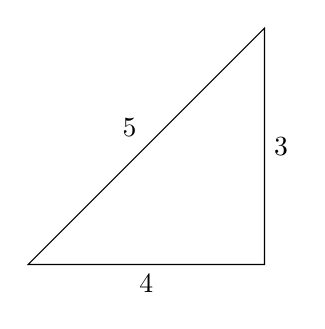
\begin{tikzpicture}
                    \draw (0,0) -- (3,0) -- (3,3) -- cycle;
                    \node at (3, 1.5) [right] {$3$};
                    \node at (1.5, 0) [below] {$4$};
                    \node at (1.5, 1.5) [above left] {$5$};
                \end{tikzpicture}
                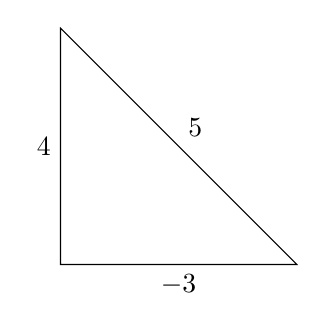
\begin{tikzpicture}
                    \draw (0,0) -- (-3,0) -- (-3,3) -- cycle;
                    \node at (-3, 1.5) [left] {$4$};
                    \node at (-1.5, 0) [below] {$-3$};
                    \node at (-1.5, 1.5) [above right] {$5$};
                \end{tikzpicture}
            \end{center}
            \begin{align*}
                \cos(A + 2B) &= \cos A \cos 2B - \sin A \sin 2B\\
                &= \cos A(1 - 2\sin^2 B) - \sin A(2\sin B \cos B)\\
                & = \dfrac{4}{5}\left(1 - 2\left(\dfrac{4}{5}\right)^2\right) - \dfrac{3}{5}\left(2\cdot\dfrac{4}{5}\cdot\left(-\dfrac{3}{5}\right)\right)\\
                & = \dfrac{44}{125} & \blacksquare
            \end{align*}
            
            \item 不许用计算机, 求 $\cos ^2 \dfrac{\pi}{8}-\cos ^2 \dfrac{3 \pi}{8}$ 的值。
            \sol{}
            \begin{align*}
                \cos^2\dfrac{\pi}{8} - \cos^2\dfrac{3\pi}{8} &= \cos^2\dfrac{\pi}{8} - \sin^2\dfrac{\pi}{8}\\
                &= \cos^2\left(\dfrac{1}{2}\cdot \dfrac{\pi}{4}\right) - \sin^2\left(\dfrac{1}{2}\cdot \dfrac{\pi}{4}\right)\\
                &= \cos\dfrac{\pi}{4} = \dfrac{\sqrt{2}}{2} & \blacksquare
            \end{align*}
        \end{enumerate}

        \item 已知 $\cos \theta+\sin \theta=a$ 及 $\cos 2 \theta=b$, 证明 $a^4-2 a^2+b^2=0$。
        
        \sol{}
        \begin{align*}
            a &= \cos \theta + \sin \theta\\
            a^2 &= \cos^2\theta + 2\sin\theta\cos\theta + \sin^2\theta\\
            &= 1 + \sin 2\theta\\
            a^4 - 2a^2 + b^2 &= (1 + \sin 2\theta)^2 - 2(1 + \sin 2\theta) + \cos^2 2\theta\\
            &= 1 + 2\sin 2\theta + \sin^2 2\theta - 2 - 2\sin 2\theta + \cos^2 2\theta\\
            &= \sin^2 2\theta + \cos^2 2\theta - 1\\
            & = 1 - 1 = 0 & \blacksquare
        \end{align*}

    \end{enumerate}

\end{document}
